\label{gettingstarted}
\section{File opening}
This tutorial will cover the basic program functionality from opening a file to fitting functions to data.
\begin{itemize}
  \item \href{http://www.stimfit.org/index.php?option=com_content&task=section&id=5&Itemid=27}{Download the Stimfit setup program}\footnote{\url{http://www.stimfit.org}} and install Stimfit on your computer.
  \item \href{http://stimfit.org/tutorial/sample.dat}{Download the sample data file}\footnote{\url{http://stimfit.org/tutorial/sample.dat}}.
  \item Open the data file: you can either double-click it from an Explorer Window, or you can start Stimfit and choose ``File'' $\rightarrow$``Open...'' from the menu.
  \item The file will be opened in a new child window, and the first trace will be displayed.
\end{itemize}

\section{Trace scaling}
\begin{itemize}
  \item If you just see scale bars, but no trace is displayed, press \keybox{F} or click the corresponding button (Fig. \ref{fittowindow}). This will fit the first trace of the active channel (plotted in black) to the screen.
  \begin{myfigure}[htb]
    \begin{center}
      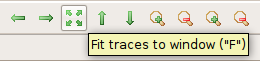
\includegraphics[scale=0.75]{./img/fittowindow.eps}
    \end{center}
    \caption{Fit traces to the window size.}
    \label{fittowindow}
  \end{myfigure}
  \item If you prefer coordinates to scale bars, you can uncheck ``View''$\rightarrow$``Scale bars'' in the menu (Fig. \ref{viewscalebars}).
  \begin{myfigure}[ht]
    \begin{center}
      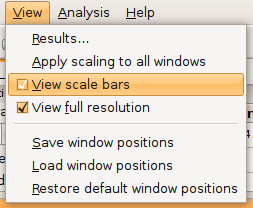
\includegraphics[scale=0.5]{./img/viewscalebars.eps}
    \end{center}
    \caption{Show coordinates rather than scale bars.}
    \label{viewscalebars}
  \end{myfigure}
  \item Fit the inactive channel (plotted in red) to the screen as well: Press \keybox{3}. The buttons labelled ``1'' and ``2'' should now both be highlighted (Fig. \ref{channelselection}). That means that any changes to the scaling will now be applied to both channels simultaneously. Press \keybox{F} again. The inactive channel (red trace) will now be fitted to the screen as well. If you want to scale channels individually, press either \keybox{1} or \keybox{2}.
  \begin{myfigure}[ht]
    \begin{center}
      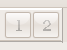
\includegraphics[scale=0.75]{./img/channelselection.eps}
    \end{center}
    \caption{Scaling applies to both channels.}
    \label{channelselection}
  \end{myfigure}
  \item Enlarge the vertical scale: Press \keybox{+}. Depending on which channel(s) you selected, the vertical scale will be enlarged by a factor of 10\%. Shrink the scale back to its original value by pressing \keybox{-}.
  \item Enlarge the time scale: Press \keybox{Ctrl} and \keybox{+} simultaneously. The time scale will be enlarged for both channels, regardless of which channel you have chosen, because Stimfit assumes that both channels have been sampled at the same time and frequency.
  \item Shrink the time scale back to its original value by pressing \keybox{Ctrl} and \keybox{-} simultaneously.
  \item Shift the trace by pressing \keybox{Ctrl} and one of the cursor (arrow) keys simultaneously.
  \item You can zoom into parts of the trace using a zoom window: Press \keybox{Z}. The zoom button (showing a magnifying glass) will be highlighted (Fig. \ref{zoom}).
  \begin{myfigure}[ht]
    \begin{center}
      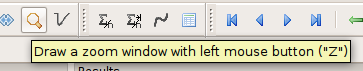
\includegraphics[scale=0.5]{./img/zoom.eps}
    \end{center}
    \caption{Setting the mouse cursor to draw zoom windows.}
    \label{zoom}
  \end{myfigure}
  \item Drag a window over the region of interest holding down the left mouse button. Release the left mouse button once you are done. When you right-click on the window, a menu will pop up showing different zoom options. Select ``Expand zoom window horizontally \& vertically'' (Fig. \ref{popupzoom}).
  \begin{myfigure}[ht]
    \begin{center}
      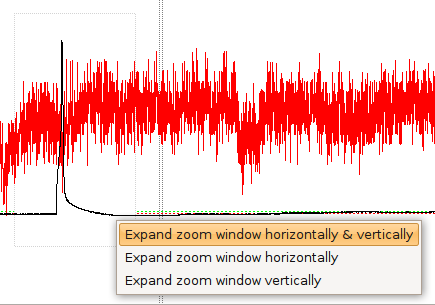
\includegraphics[scale=0.5]{./img/zoompopup.eps}
    \end{center}
    \caption{Magnifying a region of interest.}
    \label{popupzoom}
  \end{myfigure}
  \item If you can't see any trace because you zoomed in or out too much, press \keybox{F} to fit the trace to the screen again.
\end{itemize}
  \infobox{Although all commands mentioned above can be accessed with the mouse, I strongly recommend using the keyboard shortcuts; once you get used to it, the shortcuts are much faster (see p. \pageref{shortcuts} for a list).}

\section{Navigate within a file}
\begin{itemize}
  \item You can toggle through \keyindex{tracesselection}{traces!selection}{traces}traces using the \keybox{$\leftarrow$} or \keybox{$\rightarrow$} keys (\textit{without} pressing \keybox{Ctrl} at the same time). The current trace number will be displayed in the drop-down box labelled "Trace ... of ...". You can directly select a trace from this box as well (Fig. \ref{traceselection}).
  \begin{myfigure}[ht]
    \begin{center}
      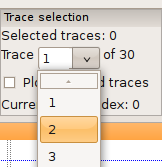
\includegraphics[scale=0.5]{./img/traceselection.eps}
    \end{center}
    \caption{Selecting a trace.}
    \label{traceselection}
  \end{myfigure}
  \item All measurements will be performed on the active channel plotted in black. You can swap \keyindex{channelindex}{channels!selection}{channels}channels by either selecting ``View''$\rightarrow$``Swap channels'' from the menu, or setting the channels in the drop-down boxes (Fig. \ref{channeldrop}).
  \begin{myfigure}[ht]
    \begin{center}
      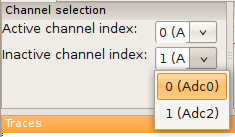
\includegraphics[scale=0.5]{./img/channelselectiondrop.eps}
    \end{center}
    \caption{Setting the active and inactive channel.}
    \label{channeldrop}
  \end{myfigure}
\end{itemize}

\section{Analyse individual events}
An ``event'' can be anything from an EPSC to an action potential. In this case, we will analyse a large spontaneous EPSC in trace no. 12 of the second channel. Navigate to trace number 12, swap channels, and zoom into the large EPSC as described above. All results are displayed in the \keyindex{results}{results table}{results table}results table (Fig. \ref{resultstable}). You can select which results to show in the table by right-clicking on one of the column or row title labels, and then selecting or unselecting the corresponding items.
  \begin{myfigure}[ht]
    \begin{center}
      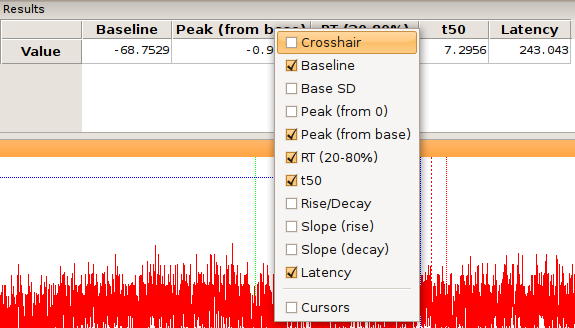
\includegraphics[scale=0.5]{./img/resultstable.eps}
    \end{center}
    \caption{Showing analysis results.}
    \label{resultstable}
  \end{myfigure}

Stimfit uses \keyindex{cursors}{cursors}{cursors}cursors to define measurement windows. Cursors are represented by vertical dashed lines extending throughout the window, similar as on an oscilloscope. For example, the \keyindex{baselineindex}{baseline}{baseline}baseline is calculated as the average of all sampling points between the two base window cursors (vertical green dashed lines). To move the cursors, press \keybox{B}. The corresponding toolbar button will be highlighted. Set the left cursor by clicking the left mouse button where you want the baseline calculation to start. Set the right cursor by clicking the right mouse button where you want the baseline calculation to end. Press \keybox{Enter}. The result of the baseline calculation is displayed in the results table, and the baseline is plotted as a horizontal green dashed line (Fig. \ref{baseline}).
  \begin{myfigure}[ht]
    \begin{center}
      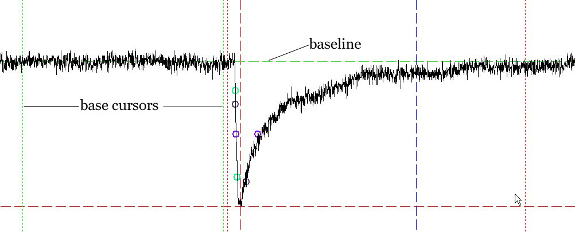
\includegraphics[width=0.7\textwidth]{./img/baseline.eps}
    \end{center}
    \caption{Setting the baseline window cursors.}
    \label{baseline}
  \end{myfigure}
\, \\ \smallskip
\infobox{You have to press \keybox{Enter} after changing any cursor position to update all calculations. Otherwise, you will see the results of your previous cursor settings. Alternatively, you can call \texttt{measure()} from the Python shell (see p. \pageref{measure}).}

The \keyindex{peakcalculation}{peak!calculation}{peak calculation}peak value will be determined between the two peak window cursors (vertical red dashed lines).  To move the cursors, press \keybox{P}. The corresponding toolbar button will be highlighted. Set the left cursor by clicking the left mouse button where you want the peak detection to start. Set the right cursor by clicking the right mouse button where you want the peak detection to end. Press \keybox{Enter}.  The result of the peak calculation is displayed in the results bar. ``Peak (from base)'' is the difference between the peak value and the baseline, and ``Peak (from 0)'' is the ``raw'' value of the peak, measured from zero, without any subtraction. A horizontal red dashed line will indicate the peak value, and a vertical dashed line will indicate the point in time when this peak value has been detected (Fig. \ref{peak}).
  \begin{myfigure}[ht]
    \begin{center}
      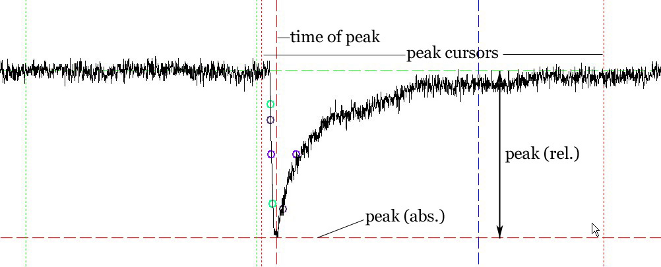
\includegraphics[width=0.7\textwidth]{./img/peak.eps}
    \end{center}
    \caption{Setting the peak window cursors.}
    \label{peak}
  \end{myfigure}

There are three ways the peak value can be calculated: \keyindex{peakdirection}{peak!direction}{peak direction}As a default, it is calculated as the maximal absolute value measured from baseline; hence, both positive- or negative-going events may be detected, whichever is larger. If you want only positive-going events to be detected,  select ``Edit''$\rightarrow$``Cursor settings'' from the menu. A dialog will appear. Select the ``Peak'' tab, and then check the ``Up'' radio button  (Fig. \ref{cursorsettings}). Click the ``Apply'' button to measure the peak using your new settings. If you only want negative-going events to be detected, select ``Down'' instead. Selecting ``Both'' resets the peak calculation to the default mode. If you want to set the peak direction from the Python shell, you can call \pyindex{setpeakdirection}{set\_peak\_direction}\pycommand{set\_peak\_direction(direction)}, where \pycommand{direction} can be one of \pycommand{"up"}, \pycommand{"down"} or \pycommand{"both"}. The Python shell will be explained in some more detail in chapter \ref{pythonshell}.
  \begin{myfigure}[ht]
    \begin{center}
      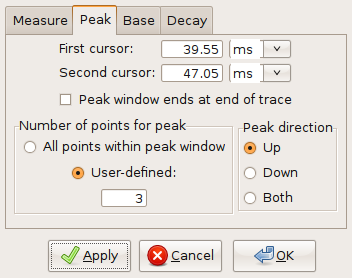
\includegraphics[scale = 0.5]{./img/cursorsettings.eps}
    \end{center}
    \caption{Setting the peak calculation properties.}
    \label{cursorsettings}
  \end{myfigure}

In case the event you want to analyse is noisy, it may be helpful to use the \keyindex{peakmovingaverage}{peak!moving average}{moving average}average of several neighbouring sampling points for the peak calculation instead of a single sampling point. A moving average algorithm will then be used to calculate the peak value. The number of sampling points can either be set in the cursor settings dialog (Fig. \ref{cursorsettings}) or from the Python shell using \pyindex{setpeakmean}{set\_peak\_mean}\pycommand{set\_peak\_mean(pts)}, where \pycommand{pts} is the number of sampling points.

Some other values describing the event can be found in the results table (Fig. \ref{overview}):
\begin{itemize}
  \item \index{rise time}``RT(20-80\%)''refers to the time required for the signal to change from 20 to 80\% of the peak value (measured from baseline), commonly called the ``20-to-80\%-risetime''.  The points corresponding to 20 and 80\% of the peak value are indicated by green circles. They are determined by linear interpolation between neighbouring sampling points.
  \item \index{half duration}``t1/2'' refers to the full width of the signal at half-maximal amplitude (measured from baseline), commonly called "half-duration". The points where the signal reaches its half-maximal amplitude are indicated by blue circles. Again, this is determined by linear interpolation between neighbouring sampling points. 
  \item ``Rise'' and ``Decay'' refer to the maximal slope during the rising and the falling phase of the signal, respectively. The corresponding points are indicated by violet circles.
  \item \index{R/D}``R/D'' is the ratio of the maximal slopes during the rising and the falling phase of the signal.
\end{itemize}

\infobox{From version 0.8.6 on, the rise time and half duration calculation is independent of the baseline and peak window cursor positions. In versions prior to 0.8.6, the baseline cursors had to precede the peak window cursors. However, the calculation of the maximal slopes of rise and decay is still restricted to the peak window.}
  \begin{myfigure}[ht]
    \begin{center}
      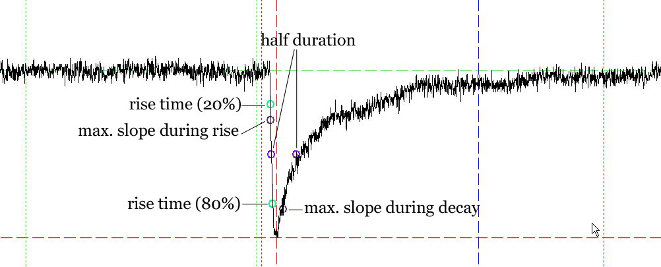
\includegraphics[width=0.7\textwidth]{./img/overview.eps}
    \end{center}
    \caption{Analysis of individual events.}
    \label{overview}
  \end{myfigure}

\section{Average calculation}
First, you have to select the traces that you want to average\keyindex{averagecalculation}{average calculation}{average calculation}: navigate through the file with the \keybox{$\leftarrow$} and \keybox{$\rightarrow$} keys (as described above), and press \keybox{S} if you want to select a trace, or click the selection button. The number of traces that you have already selected will be shown just above the trace selection drop-down box (Fig. \ref{selection}).
  \begin{myfigure}[ht]
    \begin{center}
      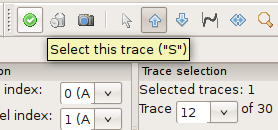
\includegraphics[scale = 0.5]{./img/selection.eps}
    \end{center}
    \caption{Trace selection.}
    \label{selection}
  \end{myfigure}
If you selected a trace accidentally, you can remove it from the selected traces list by pressing \keybox{R} or clicking the trash bin button to the right of the selection button (Fig. \ref{selection}).

Once you are done, click the "Average" button to compute the average of all selected traces (Fig. \ref{average}). A new child window will pop up showing the average. In the original child window, the average is shown as a blue trace.
  \begin{myfigure}[ht]
    \begin{center}
      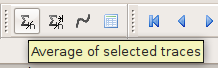
\includegraphics[scale = 0.5]{./img/average.eps}
    \end{center}
    \caption{Average calculation.}
    \label{average}
  \end{myfigure}
\, \\ \smallskip
\infobox{This is a general concept for most analysis functions: you first select traces, and the analysis will then be performed on the selected traces.}

\section{Fitting functions to data}
\index{curve fitting}\index{fitting|see{curve fitting}}\index{nonlinear regression|see{curve fitting}}
\begin{itemize}
\item Navigate to trace number 12 which contains a large spontaneous EPSC. Swap channels as described above, then zoom into the large EPSC.
\item Set the peak and baseline cursors appropriately; the peak and baseline values will be used as initial values for the fit. Don't forget to press \keybox{Enter}.
\item The function will be fitted to the data between the two fit window cursors (grey vertical dashed lines). To move the cursors, press \keybox{D} (historically, ``D'' stands for ``decay''). The corresponding button will be highlighted. Set the left cursor by clicking the left mouse button where you want the fit to start. Set the right cursor by clicking the right mouse button where you want the fit to end. Press \keybox{Enter} to confirm the cursor settings.
\item Select ``Analysis''$\rightarrow$``Fit''$\rightarrow$``Non-linear regression'' from the menu. Select a bi-exponential function (Fig. \ref{fitselection}).
\end{itemize}
  \begin{myfigure}[ht]
    \begin{center}
      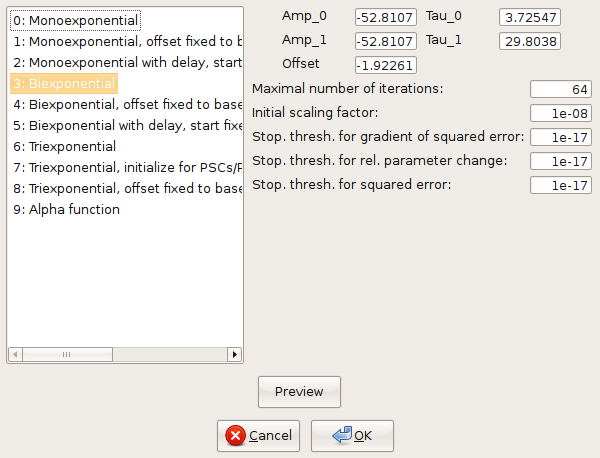
\includegraphics[scale = 0.5]{./img/fitselection.eps}
    \end{center}
    \caption{Non-linear regression settings.}
    \label{fitselection}
  \end{myfigure}
\begin{itemize}
\item The fitted function will be displayed as a thick grey line, and a table showing the best-fit parameters and the sum of squared errors (SSE) will pop up (Fig. \ref{fit}).
\end{itemize}
  \begin{myfigure}[ht]
    \begin{center}
      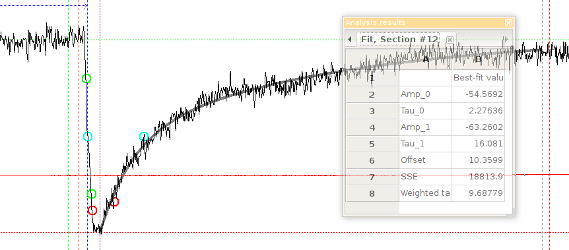
\includegraphics[width=0.7\textwidth]{./img/fit.eps}
    \end{center}
    \caption{Results of a non-linear regression using a bi-exponential function.}
    \label{fit}
  \end{myfigure}
\pycommand{\textbf{leastsq(fselect, refresh=True)}}\pyindex{leastsq}{leastsq}\\ can be called from the Python shell to fit the function with index \pycommand{fselect} to the data. \pycommand{fselect} refers to the number that you can find in front of the functions in the fit settings dialog (see Fig. \ref{fitselection}). If \pycommand{refresh=False}, the trace will not be re-drawn, wich can be useful to avoid flicker when performing a series of fits.